% =============================================================
%  Excel Transfer Tool — Premium User Manual
%  Modern, professional LaTeX layout
% =============================================================
\documentclass[11pt,a4paper]{article}

% ── Core layout ──────────────────────────────────────────────
\usepackage[a4paper,top=2.8cm, bottom=3cm,left=2.4cm, right=2.4cm,headheight=14pt]{geometry}

% ── Typography ───────────────────────────────────────────────
\usepackage[T1]{fontenc}
\usepackage[utf8]{inputenc}
\usepackage{lmodern}
\usepackage{microtype}
\usepackage{setspace}
\usepackage{letterspace}  % For \textls letter spacing
\setstretch{1.15}

% ── Graphics & color ─────────────────────────────────────────
\usepackage{graphicx}
\usepackage{float}
\usepackage[table]{xcolor}
\usepackage{tikz}
\usetikzlibrary{shadows.blur, positioning, shapes.geometric}

% ── Header / footer ──────────────────────────────────────────
\usepackage{fancyhdr}
\usepackage{lastpage}

% ── Tables ───────────────────────────────────────────────────
\usepackage{booktabs}
\usepackage{tabularx}
\usepackage{array}

% ── Lists ────────────────────────────────────────────────────
\usepackage{enumitem}

% ── Sections styling ─────────────────────────────────────────
\usepackage{titlesec}

% ── Colored boxes ────────────────────────────────────────────
\usepackage[most]{tcolorbox}

% ── Hyperlinks ───────────────────────────────────────────────
\usepackage{hyperref}

% ── Misc ─────────────────────────────────────────────────────
\usepackage{parskip}
\usepackage{mdframed}

% =============================================================
%  COLOUR PALETTE - Light Premium Professional
% =============================================================
\definecolor{PrimaryBlue}{HTML}{2C3E50}      % Deep slate - serious but not dark
\definecolor{AccentBlue}{HTML}{5D6D7E}       % Muted blue-gray
\definecolor{LightBlue}{HTML}{EBF5FB}        % Very light blue
\definecolor{Teal}{HTML}{7D8A96}             % Soft teal-gray
\definecolor{LightTeal}{HTML}{E8F0F5}        % Pale blue
\definecolor{SoftGray}{HTML}{F8F9FA}         % Off-white
\definecolor{MidGray}{HTML}{D5DBDB}          % Light gray
\definecolor{DarkText}{HTML}{34495E}         % Charcoal blue
\definecolor{MutedText}{HTML}{85929E}        % Soft gray
\definecolor{Warning}{HTML}{D68910}          % Warm amber
\definecolor{LightWarning}{HTML}{FEF9E7}     % Pale yellow
\definecolor{Danger}{HTML}{CB4335}           % Muted red
\definecolor{Success}{HTML}{27AE60}          % Fresh green
\definecolor{LightSuccess}{HTML}{EAFAF1}     % Pale green
\definecolor{White}{HTML}{FFFFFF}
\definecolor{PremiumGold}{HTML}{D4AF37}      % Elegant gold
\definecolor{ModernBlue}{HTML}{3498DB}       % Clean modern blue
\definecolor{SoftPurple}{HTML}{9B59B6}       % Elegant purple
\definecolor{LightAccent}{HTML}{F4F6F7}      % Almost white with hint of blue

% =============================================================
%  HYPERREF SETUP
% =============================================================
\hypersetup{
    colorlinks=true,
    linkcolor=AccentBlue,
    urlcolor=Teal,
    citecolor=AccentBlue,
    pdftitle={Excel Transfer Tool User Manual},
    pdfauthor={Finance Automation Team},
    bookmarksnumbered=true
}

% =============================================================
%  HEADER & FOOTER
% =============================================================
\pagestyle{fancy}
\fancyhf{}
\fancyhead[L]{%
    
\begin{tikzpicture}[baseline=(A.base)]
        \node[inner sep=0pt] (A) {%
            \textcolor{PrimaryBlue}{\textbf{\small Excel Transfer Tool}}%
        };
    \end{tikzpicture}%
}
\fancyhead[C]{\textcolor{MutedText}{\small User Manual}}
\fancyhead[R]{\textcolor{MutedText}{\small v2.0 · \today}}

\renewcommand{\headrulewidth}{0.4pt}
\renewcommand{\headrule}{\hbox to\headwidth{%
    \color{AccentBlue}\leaders\hrule height \headrulewidth\hfill}}

\fancyfoot[L]{\textcolor{MutedText}{\scriptsize Finance Automation · Internal Use Only}}
\fancyfoot[C]{}
\fancyfoot[R]{\textcolor{MutedText}{\scriptsize Page \thepage\ of \pageref{LastPage}}}

\renewcommand{\footrulewidth}{0.4pt}
\renewcommand{\footrule}{\hbox to\headwidth{%
    \color{MidGray}\leaders\hrule height \footrulewidth\hfill}}

% =============================================================
%  SECTION STYLING
% =============================================================
\titleformat{\section}{%
    \Large\bfseries\color{White}%
}{}{0em}{%
    \colorbox{PrimaryBlue}{\parbox{\dimexpr\linewidth-2\fboxsep\relax}{%
        \vspace{4pt}\hspace{6pt}%
        \Large\bfseries\color{White}%
    }}%
}

\titleformat{\subsection}{%
    \large\bfseries\color{PrimaryBlue}%
}{}{0em}{%
    \large\bfseries\color{PrimaryBlue}%
}[\vspace{-6pt}\textcolor{AccentBlue}{\rule{\linewidth}{1.5pt}}]

\titleformat{\subsubsection}{%
    \normalsize\bfseries\color{AccentBlue}%
}{}{0em}{}

% =============================================================
%  CUSTOM BOXES
% =============================================================
% Info box
\newtcolorbox{infobox}[1][Note]{
    enhanced,
    colback=LightBlue,
    colframe=AccentBlue,
    boxrule=1pt,
    arc=6pt,
    left=10pt, right=10pt, top=8pt, bottom=8pt,
    fonttitle=\bfseries\color{AccentBlue},
    title=#1,
    attach boxed title to top left={yshift=-2mm, xshift=6mm},
    boxed title style={colback=LightBlue, colframe=AccentBlue, arc=4pt}
}

% Warning box
\newtcolorbox{warningbox}[1][Warning]{
    enhanced, colback=LightWarning, colframe=Warning, boxrule=1pt, arc=6pt,
    left=10pt, right=10pt, top=8pt, bottom=8pt,
    fonttitle=\bfseries\color{Warning}, title=#1,
    attach boxed title to top left={yshift=-2mm, xshift=6mm},
    boxed title style={colback=LightWarning, colframe=Warning, arc=4pt}
}

% Success box
\newtcolorbox{successbox}[1][Success]{
    enhanced, colback=LightSuccess, colframe=Success, boxrule=1pt, arc=6pt,
    left=10pt, right=10pt, top=8pt, bottom=8pt,
    fonttitle=\bfseries\color{Success}, title=#1,
    attach boxed title to top left={yshift=-2mm, xshift=6mm},
    boxed title style={colback=LightSuccess, colframe=Success, arc=4pt}
}

% Step box
\newtcolorbox{stepbox}[1][]{
    enhanced, colback=SoftGray, colframe=MidGray, boxrule=0.8pt, arc=8pt,
    left=12pt, right=12pt, top=10pt, bottom=10pt,
    drop shadow={SoftGray!80!black}, #1
}

% Code / path box
\newtcolorbox{codebox}{
    enhanced, colback=DarkText, colframe=DarkText, boxrule=0pt, arc=4pt,
    left=10pt, right=10pt, top=6pt, bottom=6pt,
    fontupper=\ttfamily\small\color{White}
}

% Screenshot placeholder
\newcommand{\screenshot}[3][8cm]{%
\begin{figure}[H]
\centering
\begin{tikzpicture}
\node[draw=MidGray,fill=SoftGray,rounded corners=8pt,minimum width=0.88\linewidth,
      minimum height=#1,drop shadow={shadow xshift=2pt, shadow yshift=-2pt, opacity=0.15},
      align=center,font=\color{MutedText}\small] {%
    \begin{minipage}{0.75\linewidth}
    \centering\vspace{0.5cm}
    \begin{tikzpicture}
    \node[draw=MidGray, fill=MidGray, rounded corners=4pt,
          minimum width=1.2cm, minimum height=0.8cm]{};
    \end{tikzpicture}\\[6pt]
    \textcolor{MutedText}{\textit{#2}}
    \end{minipage}};
\end{tikzpicture}
\caption{#3}
\label{fig:#3}
\end{figure}}

\begin{document}

% ─────────────────────────────────────────────────────────────
%  TITLE PAGE - Light Modern Premium Design
% ─────────────────────────────────────────────────────────────
\begin{titlepage}
\newgeometry{margin=0pt}

% Light background with modern geometric art
\begin{tikzpicture}[remember picture, overlay]
% Main background - clean white
\fill[White] (current page.north west) rectangle (current page.south east);

% Modern geometric art - top right
\begin{scope}[transparency group, opacity=0.08]
\fill[ModernBlue]
    ([xshift=-6cm, yshift=-2cm]current page.north east) 
    circle (4cm);
\fill[SoftPurple]
    ([xshift=-3cm, yshift=-5cm]current page.north east) 
    circle (3cm);
\end{scope}

% Geometric shapes - left side modern art
\begin{scope}[transparency group, opacity=0.06]
\fill[PremiumGold]
    ([xshift=2cm, yshift=-8cm]current page.north west) --
    ([xshift=5cm, yshift=-8cm]current page.north west) --
    ([xshift=3.5cm, yshift=-12cm]current page.north west) -- cycle;
\fill[ModernBlue]
    ([xshift=1cm, yshift=-14cm]current page.north west) 
    rectangle ([xshift=4cm, yshift=-17cm]current page.north west);
\end{scope}

% Bottom right accent - modern angular shape
\begin{scope}[transparency group, opacity=0.05]
\fill[Teal]
    ([xshift=-8cm]current page.south east) --
    (current page.south east) --
    ([yshift=6cm]current page.south east) -- cycle;
\end{scope}

% MORE GEOMETRIC SHAPES - scattered modern art
% Top left corner squares
\begin{scope}[transparency group, opacity=0.12]
\fill[PremiumGold] ([xshift=1cm, yshift=-2cm]current page.north west) rectangle ([xshift=1.8cm, yshift=-2.8cm]current page.north west);
\fill[ModernBlue] ([xshift=2cm, yshift=-2cm]current page.north west) rectangle ([xshift=2.8cm, yshift=-2.8cm]current page.north west);
\fill[SoftPurple] ([xshift=3cm, yshift=-2cm]current page.north west) rectangle ([xshift=3.8cm, yshift=-2.8cm]current page.north west);
\end{scope}

% Right side floating squares
\begin{scope}[transparency group, opacity=0.1]
\fill[ModernBlue] ([xshift=-4cm, yshift=-10cm]current page.north east) rectangle ([xshift=-3.2cm, yshift=-10.8cm]current page.north east);
\fill[PremiumGold] ([xshift=-3cm, yshift=-11.5cm]current page.north east) rectangle ([xshift=-2.2cm, yshift=-12.3cm]current page.north east);
\fill[SoftPurple] ([xshift=-5cm, yshift=-12cm]current page.north east) rectangle ([xshift=-4.2cm, yshift=-12.8cm]current page.north east);
\end{scope}

% Bottom left scattered squares
\begin{scope}[transparency group, opacity=0.09]
\fill[PremiumGold] ([xshift=2cm, yshift=4cm]current page.south west) rectangle ([xshift=2.8cm, yshift=4.8cm]current page.south west);
\fill[ModernBlue] ([xshift=3.5cm, yshift=3cm]current page.south west) rectangle ([xshift=4.3cm, yshift=3.8cm]current page.south west);
\fill[SoftPurple] ([xshift=1cm, yshift=2.5cm]current page.south west) rectangle ([xshift=1.8cm, yshift=3.3cm]current page.south west);
\end{scope}

% Bottom center decorative squares
\begin{scope}[transparency group, opacity=0.08]
\fill[ModernBlue] ([xshift=-8cm, yshift=2cm]current page.south east) rectangle ([xshift=-7.2cm, yshift=2.8cm]current page.south east);
\fill[PremiumGold] ([xshift=-7cm, yshift=3.5cm]current page.south east) rectangle ([xshift=-6.2cm, yshift=4.3cm]current page.south east);
\end{scope}

% Thin accent lines - modern minimalist
\fill[PremiumGold, opacity=0.4]
    ([xshift=0.8cm, yshift=-4cm]current page.north west) 
    rectangle ([xshift=0.9cm, yshift=-10cm]current page.north west);
\fill[ModernBlue, opacity=0.3]
    ([xshift=1.2cm, yshift=-5cm]current page.north west) 
    rectangle ([xshift=1.25cm, yshift=-9cm]current page.north west);

% Top accent bar - subtle
\fill[LightAccent]
    (current page.north west) rectangle 
    ([yshift=-0.3cm]current page.north east);
\end{tikzpicture}

% Content positioning
\vspace*{7cm}

% Main title block - modern centered layout
\begin{center}

% Modern geometric accent above title - MORE SQUARES

\begin{tikzpicture}
\fill[PremiumGold, opacity=0.7] (0,0) rectangle (0.8,0.8);
\fill[ModernBlue, opacity=0.6] (1,0) rectangle (1.8,0.8);
\fill[SoftPurple, opacity=0.5] (2,0) rectangle (2.8,0.8);
\fill[PremiumGold, opacity=0.4] (3.2,0.3) rectangle (3.7,0.8);
\fill[ModernBlue, opacity=0.5] (4,0.1) rectangle (4.5,0.6);
\end{tikzpicture}

\vspace{1.5cm}

% Main title - elegant with spacing
{\fontsize{44}{52}\selectfont\color{PrimaryBlue}\textls[120]{\textbf{EXCEL TRANSFER TOOL}}}\\[1cm]

% Subtitle with modern styling
{\fontsize{13}{16}\selectfont\color{AccentBlue}\textsc{Technical Documentation \& User Guide}}\\[0.5cm]

% Modern divider with squares

\begin{tikzpicture}
\draw[PremiumGold, line width=1.5pt] (0,0) -- (3,0);
\fill[ModernBlue, opacity=0.6] (3.3,-0.15) rectangle (3.6,0.15);
\fill[PremiumGold, opacity=0.5] (3.7,-0.15) rectangle (4,0.15);
\draw[ModernBlue, line width=1pt, opacity=0.5] (4.2,0) -- (5.5,0);
\end{tikzpicture}

\vspace{0.8cm}

% Version badge - modern card style

\begin{tikzpicture}
\node[
    draw=MidGray,
    fill=LightAccent,
    rounded corners=6pt,
    minimum width=6cm,
    minimum height=1.8cm,
    align=center,
    drop shadow={shadow xshift=0pt, shadow yshift=-2pt, opacity=0.08}
] {%
    {\small\color{MutedText}\textsc{Version}}\\[2pt]
    {\Large\color{PrimaryBlue}\textbf{2.0}}\\[2pt]
    {\scriptsize\color{MutedText} \today}
};
\end{tikzpicture}

\vspace{2.5cm}

% Technology stack - modern pills

\begin{tikzpicture}
\node[
    draw=ModernBlue,
    fill=LightBlue,
    rounded corners=12pt,
    minimum width=2.5cm,
    minimum height=0.8cm,
    align=center
] at (0,0) {\small\color{PrimaryBlue}\textbf{Qt 6}};

\node[
    draw=SoftPurple,
    fill=White,
    rounded corners=12pt,
    minimum width=2.8cm,
    minimum height=0.8cm,
    align=center
] at (3.2,0) {\small\color{PrimaryBlue}\textbf{C++17}};

\node[
    draw=PremiumGold,
    fill=LightAccent,
    rounded corners=12pt,
    minimum width=3.2cm,
    minimum height=0.8cm,
    align=center
] at (6.8,0) {\small\color{PrimaryBlue}\textbf{OpenXML}};
\end{tikzpicture}

\vspace{3cm}

% Decorative squares before footer

\begin{tikzpicture}
\fill[ModernBlue, opacity=0.5] (0,0) rectangle (0.5,0.5);
\fill[PremiumGold, opacity=0.6] (0.7,0) rectangle (1.2,0.5);
\fill[SoftPurple, opacity=0.4] (1.4,0) rectangle (1.9,0.5);
\fill[ModernBlue, opacity=0.3] (2.1,0.1) rectangle (2.5,0.4);
\end{tikzpicture}

\vspace{0.8cm}

% Bottom metadata - clean modern footer
\begin{tikzpicture}
\node[
    text width=14cm,
    align=center,
    font=\small\color{MutedText}
] {%
    \textcolor{PrimaryBlue}{\textbf{Finance Automation Team}}\\[4pt]
    {\scriptsize Internal Use Only · Confidential Document}
};
\end{tikzpicture}

\end{center}

\restoregeometry
\end{titlepage}

\newpage
\thispagestyle{fancy}
{\hypersetup{linkcolor=DarkText}\tableofcontents}
\newpage

% =============================================================
\section{Overview}
% =============================================================

Excel Transfer Tool is a high-performance Qt/C++ desktop application that automates monthly cost-control reporting workflows. It loads Excel workbooks (XLSM/XLSX) for multiple periods, applies configurable transfer mappings, consolidates data across months, and produces clean output files—all without manual copy-paste work.

\begin{infobox}[Key Capabilities]
\begin{itemize}[leftmargin=*, itemsep=2pt]
\item Load multiple cost-control files with parallel processing (2-3x faster)
\item Apply row-level transfer mappings per month/sheet/column
\item Rolling Transfer (RT) mode for sequential month-to-month workflows
\item Support for SAP, SAP YTD, PAX, Staff, Budget, and REFI data sources
\item Quarter quick-select buttons (Q1-Q4) for rapid period selection
\item Batch cell updates with reduced lock contention
\item Automatic formula recalculation and external link cleanup
\item Export multiple selected months into consolidated output
\end{itemize}
\end{infobox}

\screenshot[6cm]{Insert full-window main dashboard screenshot here}{Application Main Dashboard}

% =============================================================
\section{Installation}
% =============================================================

\subsection{System Requirements}

\begin{center}
\rowcolors{2}{SoftGray}{White}
\begin{tabularx}{0.88\linewidth}{@{} l X @{}}
\toprule
\rowcolor{PrimaryBlue}
\textcolor{White}{\textbf{Component}} & \textcolor{White}{\textbf{Requirement}} \\
\midrule
Operating System & Windows 10 or Windows 11 (64-bit) \\
Microsoft Excel  & Excel 2016, 2019, 2021, or Microsoft 365 \\
Runtime          & Qt 6.x (bundled with executable) \\
Compiler         & Built with MSVC 2019+ / MinGW (C++17) \\
Disk Space       & Minimum 200 MB free \\
RAM              & 8 GB minimum, 16 GB recommended for 12+ months \\
\bottomrule
\end{tabularx}
\end{center}

\subsection{Setup Steps}

\begin{stepbox}
\begin{enumerate}[leftmargin=*, itemsep=6pt]
\item Extract the application folder to your preferred location (e.g.\ Desktop).
\item Launch \texttt{ExcelTransferTool.exe}.
\item On first launch, verify the default folder paths point to your network share (L: drive).
\item Ensure cost-control files follow the expected naming convention (see Appendix).
\item Verify JSON mapping files exist in the \texttt{JSON/} subfolder.
\end{enumerate}
\end{stepbox}

\screenshot[5.5cm]{Insert installation / first-launch settings screen here}{First-Launch Settings Screen}

% =============================================================
\section{Quick Start}
% =============================================================

\begin{stepbox}
\begin{enumerate}[leftmargin=*, itemsep=8pt]
\item \textbf{Select years} by checking year checkboxes (2024, 2025, 2026, etc.).
\item Click \textbf{Generate Period Rows} to create month selection cards for each year.
\item \textbf{Select months} by checking individual months or using Q1-Q4 quick-select buttons.
\item Click \textbf{LOAD Selected Periods} to load workbooks (uses parallel loading for speed).
\item Review the mapping cards that appear in the Active Mappings section.
\item Choose an action:
    \begin{itemize}[leftmargin=*, itemsep=2pt]
    \item \textbf{Execute All} — runs all checked mapping cards in sequence.
    \item \textbf{Execute RT} — runs Rolling Transfer for sequential month processing.
    \item \textbf{Export Selected Months} — consolidates multiple months into one file.
    \end{itemize}
\item Monitor progress in the status bar and progress indicator.
\item When complete, verify output files in the destination folder.
\end{enumerate}
\end{stepbox}

\screenshot[5cm]{Insert quick-start flow annotated screenshot here}{Quick Start Workflow}

% =============================================================
\section{Loading Files}
% =============================================================

\subsection{Selecting Periods}

Use the year checkboxes and month selection cards to choose periods. The application supports:

\begin{itemize}[leftmargin=*, itemsep=4pt]
\item \textbf{Individual month selection} — check specific months
\item \textbf{Quarter quick-select} — Q1 (Jan-Mar), Q2 (Apr-Jun), Q3 (Jul-Sep), Q4 (Oct-Dec)
\item \textbf{Quarter removal} — uncheck entire quarters at once
\item \textbf{Multi-year selection} — select months across multiple years simultaneously
\end{itemize}

\begin{infobox}[Tip]
Use the \textbf{Q1–Q4 quick-select buttons} at the top of the period selector to apply or remove entire quarters across all generated period rows.
\end{infobox}

\screenshot[5cm]{Insert period selector panel screenshot here}{Year and Month Period Selection}

\subsection{Loading Workbooks}

Click \textbf{LOAD Selected Periods} to open matching cost-control files. The application uses:

\begin{itemize}[leftmargin=*, itemsep=4pt]
\item \textbf{Parallel loading} with thread pool (3 concurrent files)
\item \textbf{Lazy sheet parsing} — only loads sheets when accessed
\item \textbf{ZIP entry caching} — prevents re-reading network files
\item \textbf{Progress updates} — real-time feedback during load
\end{itemize}

\begin{warningbox}[Important]
Ensure all target files are \textbf{closed in Excel} before loading. Open files may cause read errors or file locking issues.
\end{warningbox}

\screenshot[5cm]{Insert loaded files list / confirmation panel here}{Loaded Files Confirmation Panel}

% =============================================================
\section{Mapping Cards}
% =============================================================

\subsection{What is a Mapping Card?}

Each mapping card represents a transfer rule between:

\begin{itemize}[leftmargin=*, itemsep=2pt]
\item A \textbf{source} workbook, sheet, and column (where data is read from)
\item A \textbf{destination} sheet and column (where data is written to)
\item A set of \textbf{source rows} and their corresponding \textbf{destination rows}
\item Optional \textbf{row mapping} (rowMap) for summing multiple source rows into one destination
\end{itemize}

\screenshot[6cm]{Insert mapping card list screenshot here}{Mapping Cards Overview}

\subsection{Data Source Types}

The application supports multiple data source types:

\begin{center}
\rowcolors{2}{SoftGray}{White}
\begin{tabularx}{0.88\linewidth}{@{} l X @{}}
\toprule
\rowcolor{PrimaryBlue}
\textcolor{White}{\textbf{Source Type}} & \textcolor{White}{\textbf{Description}} \\
\midrule
SAP & Monthly SAP export files (MM\_YYYY.xlsx) \\
SAP YTD & Year-to-date SAP cumulative data \\
PAX & Passenger traffic data (monthly columns) \\
Staff & FTE staffing data (annual sheet per year) \\
Cost Control & Same-file transfers within cost control workbook \\
Budget & Annual budget reference columns \\
REFI & Re-forecast columns for current or prior year \\
\bottomrule
\end{tabularx}
\end{center}

\subsection{Editing Row Mappings}

Click \textbf{Edit Rows} on any card to:

\begin{itemize}[leftmargin=*, itemsep=4pt]
\item Adjust individual row numbers
\item Add new source/destination row pairs
\item Remove unused rows
\item Configure rowMap for sum operations
\end{itemize}

\screenshot[5.5cm]{Insert edit rows dialog screenshot here}{Edit Rows Dialog}

\subsection{Select All / Deselect All}

Use the \textbf{Select All / Deselect All} toggle button to quickly check or uncheck all mapping cards. Only checked cards will be executed when you click \textbf{Execute All}.

% =============================================================
\section{Rolling Transfer (RT)}
% =============================================================

\subsection{What is Rolling Transfer?}

Rolling Transfer is a specialized workflow that processes months sequentially, where each month's output becomes the input for the next month. This is used when:

\begin{itemize}[leftmargin=*, itemsep=4pt]
\item You need to "roll forward" data from one month to the next
\item Each month builds upon the previous month's calculations
\item You want to create a chain of monthly files in sequence
\end{itemize}

\subsection{How RT Works}

\begin{enumerate}[leftmargin=*, itemsep=6pt]
\item Select multiple months in chronological order
\item Click \textbf{Load RT} to validate the chain:
    \begin{itemize}[leftmargin=*, itemsep=2pt]
    \item Verifies previous month file exists for the first month
    \item Warns if destination files already exist
    \item Loads all required mappings
    \end{itemize}
\item Click \textbf{Execute RT} to run the chain:
    \begin{itemize}[leftmargin=*, itemsep=2pt]
    \item Copies previous month's file to new month's test/ folder
    \item Loads the copied file as destination
    \item Applies all mappings for that month
    \item Saves and moves to next month
    \end{itemize}
\end{enumerate}

\begin{warningbox}[RT Validation]
RT validates that the previous month's file exists before starting. If January 2026 is your first month, the December 2025 file must exist in the source folder.
\end{warningbox}

\screenshot[5cm]{Insert RT workflow diagram here}{Rolling Transfer Workflow}

% =============================================================
\section{Export Selected Months}
% =============================================================

\subsection{How It Works}

\textbf{Export Selected Months} consolidates data from multiple months into a single output workbook (the \textbf{latest selected month} file). This is used when you need to deliver a period report covering multiple months.

The process:

\begin{enumerate}[leftmargin=*, itemsep=4pt]
\item Reads each selected month's source file
\item Transfers all mapping rows into the latest month's workbook
\item Saves the combined file to the configured destination folder
\item Cleans all external links and triggers recalculation
\end{enumerate}

\screenshot[5.5cm]{Insert Export Selected Months button area screenshot here}{Export Selected Months Button}

\subsection{Running the Export}

\begin{stepbox}
\begin{enumerate}[leftmargin=*, itemsep=6pt]
\item Select all months you wish to consolidate
\item Click \textbf{LOAD Selected Periods} to load the workbooks
\item Click \textbf{Export Selected Months}
\item Monitor progress in the status bar
\item Verify the output file in the destination folder
\end{enumerate}
\end{stepbox}

\begin{infobox}[Automatic Mapping Inclusion]
The export automatically includes all mapping types (SAP, SAP YTD, PAX, Staff, Budget, REFI) for all loaded months, as long as the corresponding source workbooks are available.
\end{infobox}

\screenshot[5cm]{Insert export progress dialog screenshot here}{Export Progress and Completion}

% =============================================================
\section{Execute All Transfers}
% =============================================================

\subsection{Running All Transfers}

\textbf{Execute All} processes every checked mapping card in order. It reads each source value and writes it to the destination workbook using batch cell updates for optimal performance.

\begin{stepbox}
\begin{enumerate}[leftmargin=*, itemsep=6pt]
\item Ensure files are loaded
\item Check the mapping cards you want to execute (or use Select All)
\item Click \textbf{Execute All}
\item Monitor progress in the status bar and progress indicator
\item On completion, a summary shows total cells transferred
\end{enumerate}
\end{stepbox}

\screenshot[5cm]{Insert Execute All Transfers progress screenshot here}{All Transfers Running}

\subsection{Pause and Stop}

You can interrupt a running transfer using:

\begin{itemize}[leftmargin=*, itemsep=4pt]
\item \textbf{Pause} — temporarily halts execution, can be resumed
\item \textbf{Stop} — terminates execution immediately
\end{itemize}

\begin{warningbox}[Warning]
Stopping a transfer mid-run may leave some destination cells partially updated. Always review the output after an interrupted transfer.
\end{warningbox}

\subsection{Performance Optimizations}

The application uses several optimizations for fast execution:

\begin{itemize}[leftmargin=*, itemsep=4pt]
\item \textbf{Batch cell updates} — groups multiple cell writes into single operations
\item \textbf{Reduced lock contention} — minimizes thread synchronization overhead
\item \textbf{In-memory processing} — all operations happen in RAM before saving
\item \textbf{Lazy sheet loading} — only parses sheets when accessed
\end{itemize}

% =============================================================
\section{Saving and Finalization}
% =============================================================

After each transfer or export, the application automatically:

\begin{enumerate}[leftmargin=*, itemsep=4pt]
\item \textbf{Writes patch file} to local temp folder using miniz compression
\item \textbf{Verifies patch file} size and integrity before touching original
\item \textbf{Creates backup} by renaming original to .bak
\item \textbf{Copies patch} to final destination (network share safe)
\item \textbf{Removes backup} only after successful copy
\item \textbf{Preserves timestamps} for all ZIP entries
\item \textbf{Stores metadata} uncompressed ([Content\_Types].xml, .rels files)
\end{enumerate}

\begin{successbox}[Finalization Complete]
When finalization completes, a green status message confirms the output path and the number of cells transferred. The .bak file is automatically removed on success.
\end{successbox}

\begin{infobox}[File Safety]
If the copy operation fails, the original .bak file is automatically restored, ensuring no data loss. The patch file is left in the temp folder for inspection.
\end{infobox}

\screenshot[4.5cm]{Insert final status bar success message screenshot here}{Finalization Success Message}

% =============================================================
\section{Troubleshooting}
% =============================================================

\subsection{Files Not Saving}

\begin{warningbox}[Symptom]
Execute All completes but output files are unchanged or missing.
\end{warningbox}

\textbf{Checklist:}

\begin{itemize}[leftmargin=*, itemsep=4pt]
\item Check debug log for "miniz finalize failed" or "patch file missing"
\item Verify destination file is \textbf{closed in Excel}
\item Ensure temp folder (C:\textbackslash{}Users\textbackslash{}\{user\}\textbackslash{}AppData\textbackslash{}Local\textbackslash{}Temp) is writable
\item Check disk space on both temp drive and network share
\item Look for .bak files — if present, copy failed and original was restored
\end{itemize}

\subsection{Empty Cells After Export}

\begin{warningbox}[Symptom]
Cells that should contain SAP, PAX, or Staff values appear blank after export.
\end{warningbox}

\textbf{Checklist:}

\begin{itemize}[leftmargin=*, itemsep=4pt]
\item Confirm destination file is \textbf{closed in Excel} before exporting
\item Verify each month's source files (SAP, PAX, Staff) are available and loaded
\item Check the debug console for "file missing" or "sheet not found" messages
\item Ensure JSON mapping files have correct sheet names (case-sensitive)
\end{itemize}

\subsection{Slow Loading Performance}

\begin{itemize}[leftmargin=*, itemsep=4pt]
\item Verify network connection to L: drive is stable
\item Check if other users are accessing the same files
\item Consider reducing thread pool size in loadworker.cpp (line 50) from 3 to 2
\item Close unnecessary applications to free RAM
\end{itemize}

\subsection{File Not Found}

\begin{itemize}[leftmargin=*, itemsep=4pt]
\item Verify source folder path points to correct network location
\item Confirm file follows naming convention: \texttt{Cost Control ZAG MM\_YYYY\_working.xlsm}
\item Check if file is in test/ subfolder vs root folder
\item Ensure file has not been moved, renamed, or locked by another user
\end{itemize}

\subsection{Mapping Card Missing}

\begin{itemize}[leftmargin=*, itemsep=4pt]
\item Open the relevant JSON file (mappings.json, mappings\_old.json, pax.json, staff.json, etc.)
\item Confirm the target month/year entry exists
\item Verify sheet names match exactly (case-sensitive)
\item Check that source\_file\_type is correctly set (sap, sap\_ytd, pax, staff, cost\_control)
\end{itemize}

\subsection{RT Validation Fails}

\begin{itemize}[leftmargin=*, itemsep=4pt]
\item Ensure previous month's file exists (e.g., Dec 2025 for Jan 2026 RT)
\item Check that months are selected in chronological order
\item Verify destination test/ folders exist or can be created
\item Review RT validation messages in the status bar
\end{itemize}

% =============================================================
\section{Frequently Asked Questions}
% =============================================================

\begin{stepbox}
\textbf{Q: Can I export more than two months into a single file?}\\
A: Yes. Select all desired months, load them, then click \textbf{Export Selected Months}. All months are consolidated into the latest month's file.
\end{stepbox}

\vspace{0.4cm}

\begin{stepbox}
\textbf{Q: What's the difference between Execute All and Execute RT?}\\
A: \textbf{Execute All} processes all checked mappings independently. \textbf{Execute RT} processes months sequentially, where each month's output becomes the next month's input.
\end{stepbox}

\vspace{0.4cm}

\begin{stepbox}
\textbf{Q: Do I need to keep Excel open while the app runs?}\\
A: No. The app handles file I/O directly using OpenXML (ZIP) parsing. Excel is never launched during operation.
\end{stepbox}

\vspace{0.4cm}

\begin{stepbox}
\textbf{Q: Can I customize which rows are transferred?}\\
A: Yes. Use the \textbf{Edit Rows} button on each mapping card to adjust source and destination row numbers, or edit the JSON files directly.
\end{stepbox}

\vspace{0.4cm}

\begin{stepbox}
\textbf{Q: How do I add a new mapping type?}\\
A: Create or edit the appropriate JSON file in the JSON/ folder. The app automatically loads all JSON files on startup. Restart the app after editing JSON files.
\end{stepbox}

\vspace{0.4cm}

\begin{stepbox}
\textbf{Q: Why is parallel loading limited to 3 files?}\\
A: Large XLSM files (10-50MB) cause memory pressure when loaded in parallel. The thread pool limit of 3 balances speed with stability. This can be adjusted in loadworker.cpp if you have more RAM.
\end{stepbox}

\vspace{0.4cm}

\begin{stepbox}
\textbf{Q: What happens to external links in the output file?}\\
A: External links are automatically broken after each export to ensure the output file is self-contained and opens cleanly in Excel.
\end{stepbox}

% =============================================================
\section{Appendix}
% =============================================================

\subsection{File Naming Convention}

Cost-control files must follow this naming pattern:

\begin{codebox}
Cost Control ZAG \{MM\}\_\{YYYY\}\_working.xlsm
\end{codebox}

\textbf{Examples:}

\begin{center}
\rowcolors{2}{SoftGray}{White}
\begin{tabularx}{0.88\linewidth}{@{} l X @{}}
\toprule
\rowcolor{PrimaryBlue}
\textcolor{White}{\textbf{Month}} & \textcolor{White}{\textbf{Filename}} \\
\midrule
January 2026   & \texttt{Cost Control ZAG 01\_2026\_working.xlsm} \\
June 2026      & \texttt{Cost Control ZAG 06\_2026\_working.xlsm} \\
August 2026    & \texttt{Cost Control ZAG 08\_2026\_working.xlsm} \\
December 2026  & \texttt{Cost Control ZAG 12\_2026\_working.xlsm} \\
\bottomrule
\end{tabularx}
\end{center}

\textbf{SAP Files:}

\begin{codebox}
\{MM\}\_\{YYYY\}.xlsx
\end{codebox}

\textbf{PAX Files:}

\begin{codebox}
TRAFFIC mott \{YYYY\}.xlsx
\end{codebox}

\textbf{Staff Files:}

\begin{codebox}
\{YYYY\} FTE.xlsx
\end{codebox}

\subsection{Mapping JSON Structure}

\subsubsection{Standard Mapping (mappings.json)}

\begin{codebox}
\{\\
\quad "source\_sheet": "\{year\}",\\
\quad "source\_column": "C",\\
\quad "dest\_sheet": "MZLZ Consolidated",\\
\quad "rowMap": \{\\
\quad\quad "10": 5,\\
\quad\quad "11": [6, 7]\\
\quad \},\\
\quad "month\_mappings": [\\
\quad\quad \{"month": "January", "source\_column": "C", "dest\_column": "G"\},\\
\quad\quad \{"month": "February", "source\_column": "C", "dest\_column": "W"\}\\
\quad ]\\
\}
\end{codebox}

\subsubsection{PAX Mapping (pax.json)}

\begin{codebox}
\{\\
\quad "source": \{\\
\quad\quad "sheet": "TRAFFIC mott 2025",\\
\quad\quad "source\_rows": [19, 34, 81]\\
\quad \},\\
\quad "dest": \{\\
\quad\quad "sheet": "MZLZ Consolidated",\\
\quad\quad "dest\_rows": [5, 7, 8]\\
\quad \},\\
\quad "month\_mappings": [\\
\quad\quad \{"month": "January", "source\_column": "G", "dest\_column": "G"\}\\
\quad ]\\
\}
\end{codebox}

\subsubsection{Staff Mapping (staff.json)}

\begin{codebox}
\{\\
\quad "source": \{\\
\quad\quad "sheet": "\{year\} FTE",\\
\quad\quad "row": 33\\
\quad \},\\
\quad "dest": \{\\
\quad\quad "sheet": "MZLZ Consolidated",\\
\quad\quad "row": 16\\
\quad \},\\
\quad "month\_mappings": [\\
\quad\quad \{"month": "January", "source\_column": "D", "dest\_column": "G"\}\\
\quad ]\\
\}
\end{codebox}

\subsection{Keyboard Shortcuts}

\begin{center}
\rowcolors{2}{SoftGray}{White}
\begin{tabularx}{0.88\linewidth}{@{} l X @{}}
\toprule
\rowcolor{PrimaryBlue}
\textcolor{White}{\textbf{Shortcut}} & \textcolor{White}{\textbf{Action}} \\
\midrule
\texttt{Ctrl + L} & Load Selected Periods \\
\texttt{Ctrl + E} & Execute All Transfers \\
\texttt{Ctrl + R} & Execute Rolling Transfer \\
\texttt{Ctrl + X} & Export Selected Months \\
\texttt{Escape}   & Stop running transfer \\
\texttt{F5}       & Refresh mapping cards \\
\bottomrule
\end{tabularx}
\end{center}

\subsection{Technical Architecture}

\begin{center}
\rowcolors{2}{SoftGray}{White}
\begin{tabularx}{0.88\linewidth}{@{} l X @{}}
\toprule
\rowcolor{PrimaryBlue}
\textcolor{White}{\textbf{Component}} & \textcolor{White}{\textbf{Technology}} \\
\midrule
UI Framework      & Qt 6.x (Widgets) \\
Language          & C++17 \\
Compiler          & MSVC 2019+ / MinGW \\
Excel Parsing     & OpenXML (ZIP + XML) \\
Compression       & miniz (embedded) \\
Threading         & QThread, QThreadPool, QtConcurrent \\
JSON Parsing      & Qt JSON (QJsonDocument) \\
File I/O          & Qt File API + QZipReader/Writer \\
\bottomrule
\end{tabularx}
\end{center}

\subsection{Performance Characteristics}

\begin{center}
\rowcolors{2}{SoftGray}{White}
\begin{tabularx}{0.88\linewidth}{@{} l X @{}}
\toprule
\rowcolor{PrimaryBlue}
\textcolor{White}{\textbf{Operation}} & \textcolor{White}{\textbf{Performance}} \\
\midrule
Load 12 months (sequential)  & ~96 seconds \\
Load 12 months (parallel)    & ~32 seconds (3x faster) \\
Transfer 1000 cells (batch)  & ~0.5 seconds \\
Save 50MB XLSM file          & ~3-5 seconds \\
RT chain (6 months)          & ~2-3 minutes \\
\bottomrule
\end{tabularx}
\end{center}

\subsection{Support}

For technical issues, feature requests, or mapping configuration help, contact the internal Finance Automation support team.

\vspace{1cm}

\begin{center}
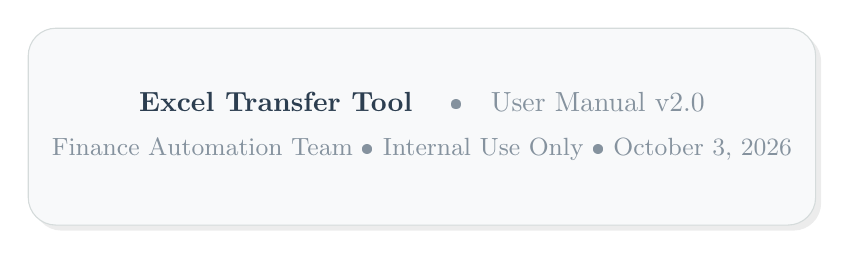
\begin{tikzpicture}
\node[draw=MidGray,fill=SoftGray,rounded corners=10pt,
      minimum width=10cm,minimum height=2.5cm,
      drop shadow={shadow xshift=2pt, shadow yshift=-2pt, opacity=0.15},
      align=center] {%
    \textcolor{PrimaryBlue}{\textbf{Excel Transfer Tool}} 
    \quad\textcolor{MutedText}{\textbullet}\quad
    \textcolor{MutedText}{User Manual v2.0}\\[4pt]
    \textcolor{MutedText}{\small Finance Automation Team \textbullet\ Internal Use Only \textbullet\ \today}};
\end{tikzpicture}
\end{center}

\end{document}
